\hypertarget{point_8c}{
\section{Referencia del Archivo point.c}
\label{point_8c}\index{point.c@{point.c}}
}


\subsection{Descripci\'{o}n detallada}
En este archivo definimos las funciones utilizadas por el objeto punto. 

Definici\'{o}n en el archivo \hyperlink{point_8c-source}{point.c}.

{\tt \#include \char`\"{}point.h\char`\"{}}\par


Dependencia gr\'{a}fica adjunta para point.c:\begin{figure}[H]
\begin{center}
\leavevmode
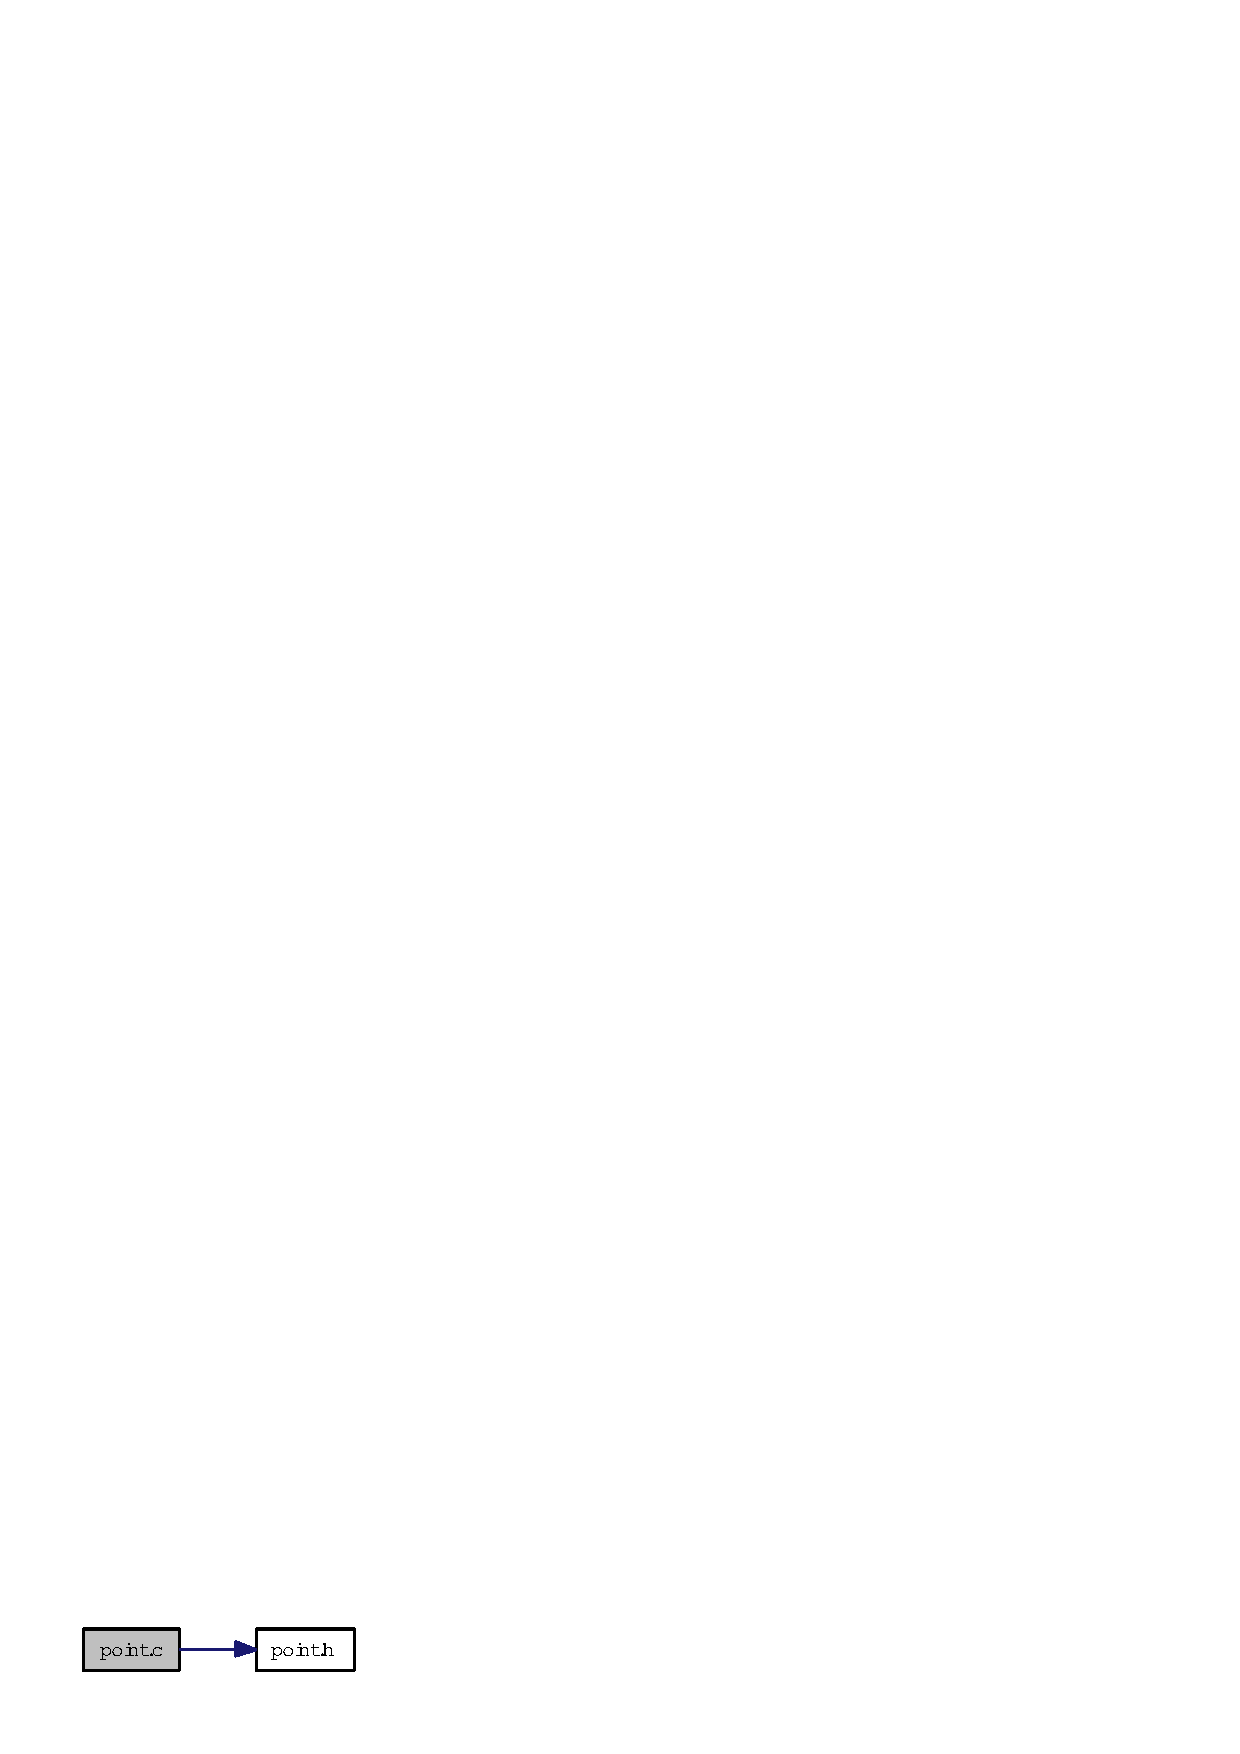
\includegraphics[width=87pt]{point_8c__incl}
\end{center}
\end{figure}
\subsection*{Funciones}
\begin{CompactItemize}
\item 
float \hyperlink{group__geometry_ga7ae8d919209fea43e8a61215398bbbe_ga7ae8d919209fea43e8a61215398bbbe}{point\_\-dot} (\hyperlink{struct__point}{point} $\ast$a, \hyperlink{struct__point}{point} $\ast$b, \hyperlink{struct__point}{point} $\ast$c)
\item 
float \hyperlink{group__geometry_gb97527165a510655ee37cd3ccfa8d932_gb97527165a510655ee37cd3ccfa8d932}{point\_\-cross} (\hyperlink{struct__point}{point} $\ast$a, \hyperlink{struct__point}{point} $\ast$b, \hyperlink{struct__point}{point} $\ast$c)
\end{CompactItemize}
